% Options for packages loaded elsewhere
\PassOptionsToPackage{unicode}{hyperref}
\PassOptionsToPackage{hyphens}{url}
%
\documentclass[
]{article}
\usepackage{amsmath,amssymb}
\usepackage{iftex}
\ifPDFTeX
  \usepackage[T1]{fontenc}
  \usepackage[utf8]{inputenc}
  \usepackage{textcomp} % provide euro and other symbols
\else % if luatex or xetex
  \usepackage{unicode-math} % this also loads fontspec
  \defaultfontfeatures{Scale=MatchLowercase}
  \defaultfontfeatures[\rmfamily]{Ligatures=TeX,Scale=1}
\fi
\usepackage{lmodern}
\ifPDFTeX\else
  % xetex/luatex font selection
\fi
% Use upquote if available, for straight quotes in verbatim environments
\IfFileExists{upquote.sty}{\usepackage{upquote}}{}
\IfFileExists{microtype.sty}{% use microtype if available
  \usepackage[]{microtype}
  \UseMicrotypeSet[protrusion]{basicmath} % disable protrusion for tt fonts
}{}
\makeatletter
\@ifundefined{KOMAClassName}{% if non-KOMA class
  \IfFileExists{parskip.sty}{%
    \usepackage{parskip}
  }{% else
    \setlength{\parindent}{0pt}
    \setlength{\parskip}{6pt plus 2pt minus 1pt}}
}{% if KOMA class
  \KOMAoptions{parskip=half}}
\makeatother
\usepackage{xcolor}
\usepackage[margin=1in]{geometry}
\usepackage{color}
\usepackage{fancyvrb}
\newcommand{\VerbBar}{|}
\newcommand{\VERB}{\Verb[commandchars=\\\{\}]}
\DefineVerbatimEnvironment{Highlighting}{Verbatim}{commandchars=\\\{\}}
% Add ',fontsize=\small' for more characters per line
\usepackage{framed}
\definecolor{shadecolor}{RGB}{248,248,248}
\newenvironment{Shaded}{\begin{snugshade}}{\end{snugshade}}
\newcommand{\AlertTok}[1]{\textcolor[rgb]{0.94,0.16,0.16}{#1}}
\newcommand{\AnnotationTok}[1]{\textcolor[rgb]{0.56,0.35,0.01}{\textbf{\textit{#1}}}}
\newcommand{\AttributeTok}[1]{\textcolor[rgb]{0.13,0.29,0.53}{#1}}
\newcommand{\BaseNTok}[1]{\textcolor[rgb]{0.00,0.00,0.81}{#1}}
\newcommand{\BuiltInTok}[1]{#1}
\newcommand{\CharTok}[1]{\textcolor[rgb]{0.31,0.60,0.02}{#1}}
\newcommand{\CommentTok}[1]{\textcolor[rgb]{0.56,0.35,0.01}{\textit{#1}}}
\newcommand{\CommentVarTok}[1]{\textcolor[rgb]{0.56,0.35,0.01}{\textbf{\textit{#1}}}}
\newcommand{\ConstantTok}[1]{\textcolor[rgb]{0.56,0.35,0.01}{#1}}
\newcommand{\ControlFlowTok}[1]{\textcolor[rgb]{0.13,0.29,0.53}{\textbf{#1}}}
\newcommand{\DataTypeTok}[1]{\textcolor[rgb]{0.13,0.29,0.53}{#1}}
\newcommand{\DecValTok}[1]{\textcolor[rgb]{0.00,0.00,0.81}{#1}}
\newcommand{\DocumentationTok}[1]{\textcolor[rgb]{0.56,0.35,0.01}{\textbf{\textit{#1}}}}
\newcommand{\ErrorTok}[1]{\textcolor[rgb]{0.64,0.00,0.00}{\textbf{#1}}}
\newcommand{\ExtensionTok}[1]{#1}
\newcommand{\FloatTok}[1]{\textcolor[rgb]{0.00,0.00,0.81}{#1}}
\newcommand{\FunctionTok}[1]{\textcolor[rgb]{0.13,0.29,0.53}{\textbf{#1}}}
\newcommand{\ImportTok}[1]{#1}
\newcommand{\InformationTok}[1]{\textcolor[rgb]{0.56,0.35,0.01}{\textbf{\textit{#1}}}}
\newcommand{\KeywordTok}[1]{\textcolor[rgb]{0.13,0.29,0.53}{\textbf{#1}}}
\newcommand{\NormalTok}[1]{#1}
\newcommand{\OperatorTok}[1]{\textcolor[rgb]{0.81,0.36,0.00}{\textbf{#1}}}
\newcommand{\OtherTok}[1]{\textcolor[rgb]{0.56,0.35,0.01}{#1}}
\newcommand{\PreprocessorTok}[1]{\textcolor[rgb]{0.56,0.35,0.01}{\textit{#1}}}
\newcommand{\RegionMarkerTok}[1]{#1}
\newcommand{\SpecialCharTok}[1]{\textcolor[rgb]{0.81,0.36,0.00}{\textbf{#1}}}
\newcommand{\SpecialStringTok}[1]{\textcolor[rgb]{0.31,0.60,0.02}{#1}}
\newcommand{\StringTok}[1]{\textcolor[rgb]{0.31,0.60,0.02}{#1}}
\newcommand{\VariableTok}[1]{\textcolor[rgb]{0.00,0.00,0.00}{#1}}
\newcommand{\VerbatimStringTok}[1]{\textcolor[rgb]{0.31,0.60,0.02}{#1}}
\newcommand{\WarningTok}[1]{\textcolor[rgb]{0.56,0.35,0.01}{\textbf{\textit{#1}}}}
\usepackage{graphicx}
\makeatletter
\def\maxwidth{\ifdim\Gin@nat@width>\linewidth\linewidth\else\Gin@nat@width\fi}
\def\maxheight{\ifdim\Gin@nat@height>\textheight\textheight\else\Gin@nat@height\fi}
\makeatother
% Scale images if necessary, so that they will not overflow the page
% margins by default, and it is still possible to overwrite the defaults
% using explicit options in \includegraphics[width, height, ...]{}
\setkeys{Gin}{width=\maxwidth,height=\maxheight,keepaspectratio}
% Set default figure placement to htbp
\makeatletter
\def\fps@figure{htbp}
\makeatother
\setlength{\emergencystretch}{3em} % prevent overfull lines
\providecommand{\tightlist}{%
  \setlength{\itemsep}{0pt}\setlength{\parskip}{0pt}}
\setcounter{secnumdepth}{-\maxdimen} % remove section numbering
\ifLuaTeX
  \usepackage{selnolig}  % disable illegal ligatures
\fi
\usepackage{bookmark}
\IfFileExists{xurl.sty}{\usepackage{xurl}}{} % add URL line breaks if available
\urlstyle{same}
\hypersetup{
  pdftitle={Market basket Analysis},
  pdfauthor={Soheil Garfami},
  hidelinks,
  pdfcreator={LaTeX via pandoc}}

\title{Market basket Analysis}
\author{Soheil Garfami}
\date{2024-08-19}

\begin{document}
\maketitle

{
\setcounter{tocdepth}{2}
\tableofcontents
}
\section{\texorpdfstring{\textbf{Introduction}}{Introduction}}\label{introduction}

Hi! In this kernel we are going to use the \textbf{Apriori algorithm} to
perform a \textbf{Market Basket Analysis}. It's a technique used by
large retailers to uncover associations between items. It works by
looking for combinations of items that occur together frequently in
transactions, providing information to understand the purchase behavior.
The outcome of this type of technique is, in simple terms, a set of
\textbf{rules} that can be understood as \textbf{``if this, then
that''}.

\subsubsection{Key Objectives}\label{key-objectives}

\textbf{\emph{Market Basket Analysis \& Association Rules}}

In this section we use association rules and the a priori algorithm to
identify purchase patterns and answer the following questions:

\begin{itemize}
\item
  Do customers purchase items together frequently and which products are
  most often purchased together ?
\item
  Can we use this information to recommend other products based on a
  customer's cart ?
\end{itemize}

\subsubsection{Importing the data}\label{importing-the-data}

First, let's import the required libraries.

\begin{Shaded}
\begin{Highlighting}[]
\FunctionTok{library}\NormalTok{(arules)}
\FunctionTok{library}\NormalTok{(arulesViz)}
\FunctionTok{library}\NormalTok{(tidyverse)}
\FunctionTok{library}\NormalTok{(ggplot2)}
\FunctionTok{library}\NormalTok{(DataExplorer)}
\FunctionTok{library}\NormalTok{(gridExtra)}
\end{Highlighting}
\end{Shaded}

let's see the data set that we built by joining all datasets

\begin{Shaded}
\begin{Highlighting}[]
\NormalTok{JOINED }\OtherTok{\textless{}{-}} \FunctionTok{read.csv}\NormalTok{(}\StringTok{"data/JOINED.csv"}\NormalTok{)}
\FunctionTok{head}\NormalTok{(JOINED)}
\end{Highlighting}
\end{Shaded}

\begin{verbatim}
##   order_id product_id add_to_cart_order reordered user_id eval_set order_number
## 1        1      49302                 1         1  112108    train            4
## 2        1      11109                 2         1  112108    train            4
## 3        1      10246                 3         0  112108    train            4
## 4        1      49683                 4         0  112108    train            4
## 5        1      43633                 5         1  112108    train            4
## 6        1      13176                 6         0  112108    train            4
##   order_dow order_hour_of_day days_since_prior_order
## 1         4                10                      9
## 2         4                10                      9
## 3         4                10                      9
## 4         4                10                      9
## 5         4                10                      9
## 6         4                10                      9
##                                    product_name aisle_id department_id
## 1                              Bulgarian Yogurt      120            16
## 2 Organic 4% Milk Fat Whole Milk Cottage Cheese      108            16
## 3                         Organic Celery Hearts       83             4
## 4                                Cucumber Kirby       83             4
## 5          Lightly Smoked Sardines in Olive Oil       95            15
## 6                        Bag of Organic Bananas       24             4
##                  aisle   department
## 1               yogurt   dairy eggs
## 2 other creams cheeses   dairy eggs
## 3     fresh vegetables      produce
## 4     fresh vegetables      produce
## 5  canned meat seafood canned goods
## 6         fresh fruits      produce
\end{verbatim}

To apply the \texttt{Apriori} algorithm in
\texttt{market\ basket\ analysis}, we need to have a
\textbf{transactions} dataset. We can import the dataset in the required
transaction format using the \texttt{arules} library. For this, we'll
need the columns for transaction ID and product name.

\begin{Shaded}
\begin{Highlighting}[]
\NormalTok{JOINED[}\DecValTok{1}\NormalTok{,}\FunctionTok{c}\NormalTok{(}\DecValTok{1}\NormalTok{,}\DecValTok{11}\NormalTok{)]}
\end{Highlighting}
\end{Shaded}

\begin{verbatim}
##   order_id     product_name
## 1        1 Bulgarian Yogurt
\end{verbatim}

As you can see, the \texttt{transactionId} and \texttt{productName}
columns are in positions 1 and 11, respectively.

let's imprort the dataset as transactions. (columns 1 and 11)

\begin{Shaded}
\begin{Highlighting}[]
\FunctionTok{rm}\NormalTok{(JOINED)}
\NormalTok{trans }\OtherTok{\textless{}{-}} \FunctionTok{read.transactions}\NormalTok{(}\StringTok{"data/JOINED.csv"}\NormalTok{ , }\AttributeTok{format =} \StringTok{"single"}\NormalTok{ , }\AttributeTok{sep =} \StringTok{","}\NormalTok{ , }\AttributeTok{cols =} \FunctionTok{c}\NormalTok{(}\DecValTok{1}\NormalTok{ ,}\DecValTok{11}\NormalTok{))}
\NormalTok{trans}
\end{Highlighting}
\end{Shaded}

\begin{verbatim}
## transactions in sparse format with
##  131210 transactions (rows) and
##  39124 items (columns)
\end{verbatim}

let's see the first transaction

\begin{Shaded}
\begin{Highlighting}[]
\FunctionTok{inspect}\NormalTok{(trans[}\DecValTok{1}\NormalTok{])}
\end{Highlighting}
\end{Shaded}

\begin{verbatim}
##     items                                            transactionID
## [1] {Bag of Organic Bananas,                                      
##      Bulgarian Yogurt,                                            
##      Cucumber Kirby,                                              
##      Lightly Smoked Sardines in Olive Oil,                        
##      Organic 4% Milk Fat Whole Milk Cottage Cheese,               
##      Organic Celery Hearts,                                       
##      Organic Hass Avocado,                                        
##      Organic Whole String Cheese}                                1
\end{verbatim}

With the \texttt{itemFrequencyPlot}, we can again visualize a graph of
the most popular products.

\begin{Shaded}
\begin{Highlighting}[]
\FunctionTok{itemFrequencyPlot}\NormalTok{(trans ,}\AttributeTok{topN=}\DecValTok{10}\NormalTok{ , }\AttributeTok{type=}\StringTok{"absolute"}\NormalTok{ ,}\AttributeTok{col=}\StringTok{"lightcyan2"}\NormalTok{,}\AttributeTok{xlab=}\StringTok{"Item name"}\NormalTok{, }
                  \AttributeTok{ylab=}\StringTok{"Frequency (absolute)"}\NormalTok{, }\AttributeTok{main=}\StringTok{"Absolute Item Frequency Plot"}\NormalTok{)}
\end{Highlighting}
\end{Shaded}

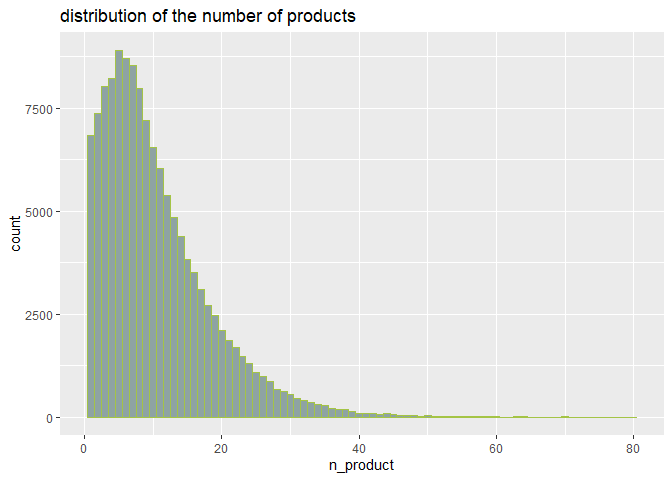
\includegraphics{Market_basket_analysis_files/figure-latex/unnamed-chunk-6-1.pdf}

\section{\texorpdfstring{\textbf{Selecting the Optimal Values for
Parameters}}{Selecting the Optimal Values for Parameters}}\label{selecting-the-optimal-values-for-parameters}

The Apriori algorithm generates association rules for a given dataset.
An association rule suggests that if item A occurs, then item B is
likely to occur with a certain probability.

To extract these rules using the Apriori algorithm, there are three key
arguments that are crucial for obtaining the best rules:

\begin{itemize}
\tightlist
\item
  \textbf{Support}: Indicates how frequently the itemset appears in the
  dataset.
\item
  \textbf{Confidence}: Reflects how often the rule has been found to be
  true.
\item
  \textbf{Lift}: Represents the ratio of the observed support to that
  expected if X and Y were independent. If the lift is greater than 1,
  it indicates the strength of the relationship between the two items,
  showing how dependent they are on each other.
\end{itemize}

Now, we will use the \texttt{gridExtra} package to build different rules
with varying parameters and plot them to determine which set of rules is
the most suitable.

\begin{Shaded}
\begin{Highlighting}[]
\CommentTok{\# Support and confidence values}
\NormalTok{supportLevels }\OtherTok{\textless{}{-}} \FunctionTok{c}\NormalTok{( }\FloatTok{0.05}\NormalTok{, }\FloatTok{0.01}\NormalTok{, }\FloatTok{0.005}\NormalTok{ , }\FloatTok{0.001}\NormalTok{)}
\NormalTok{confidenceLevels }\OtherTok{\textless{}{-}} \FunctionTok{c}\NormalTok{(  }\FloatTok{0.7}\NormalTok{, }\FloatTok{0.6}\NormalTok{, }\FloatTok{0.5}\NormalTok{, }\FloatTok{0.4}\NormalTok{, }\FloatTok{0.3}\NormalTok{, }\FloatTok{0.2}\NormalTok{, }\FloatTok{0.1}\NormalTok{ , }\FloatTok{0.05}\NormalTok{ , }\FloatTok{0.1}\NormalTok{)}

\CommentTok{\# Empty integers }
\NormalTok{rules\_sup5 }\OtherTok{\textless{}{-}} \FunctionTok{integer}\NormalTok{(}\AttributeTok{length=}\DecValTok{9}\NormalTok{)}
\NormalTok{rules\_sup1 }\OtherTok{\textless{}{-}} \FunctionTok{integer}\NormalTok{(}\AttributeTok{length=}\DecValTok{9}\NormalTok{)}
\NormalTok{rules\_sup0}\FloatTok{.5} \OtherTok{\textless{}{-}} \FunctionTok{integer}\NormalTok{(}\AttributeTok{length=}\DecValTok{9}\NormalTok{)}
\NormalTok{rules\_sup0}\FloatTok{.1} \OtherTok{\textless{}{-}} \FunctionTok{integer}\NormalTok{(}\AttributeTok{length=}\DecValTok{9}\NormalTok{)}
\end{Highlighting}
\end{Shaded}

We will test \texttt{support\ values} of 5, 1, 0.5, and 0.1, along with
\texttt{confidence\ values} of 0.7, 0.6, 0.5, 0.4, 0.3, 0.2, 0.1, 0.05,
and 0.01 to determine which combination of these two parameters works
best together.

\begin{Shaded}
\begin{Highlighting}[]
\CommentTok{\# Apriori algorithm with a support level of 5\%}
\ControlFlowTok{for}\NormalTok{ (i }\ControlFlowTok{in} \DecValTok{1}\SpecialCharTok{:}\FunctionTok{length}\NormalTok{(confidenceLevels)) \{}
  
\NormalTok{  rules\_sup5[i] }\OtherTok{\textless{}{-}} \FunctionTok{length}\NormalTok{(}\FunctionTok{apriori}\NormalTok{(trans, }\AttributeTok{parameter=}\FunctionTok{list}\NormalTok{(}\AttributeTok{sup=}\NormalTok{supportLevels[}\DecValTok{1}\NormalTok{], }
                                                         \AttributeTok{conf=}\NormalTok{confidenceLevels[i],}\AttributeTok{target=}\StringTok{"rules"}\NormalTok{), }
                                \AttributeTok{control =} \FunctionTok{list}\NormalTok{(}\AttributeTok{verbose =} \ConstantTok{FALSE}\NormalTok{)))}
\NormalTok{\}}

\CommentTok{\# Apriori algorithm with a support level of 1\%}
\ControlFlowTok{for}\NormalTok{ (i }\ControlFlowTok{in} \DecValTok{1}\SpecialCharTok{:}\FunctionTok{length}\NormalTok{(confidenceLevels))\{}
  
\NormalTok{  rules\_sup1[i] }\OtherTok{\textless{}{-}} \FunctionTok{length}\NormalTok{(}\FunctionTok{apriori}\NormalTok{(trans, }\AttributeTok{parameter=}\FunctionTok{list}\NormalTok{(}\AttributeTok{sup=}\NormalTok{supportLevels[}\DecValTok{2}\NormalTok{], }
                                                        \AttributeTok{conf=}\NormalTok{confidenceLevels[i], }\AttributeTok{target=}\StringTok{"rules"}\NormalTok{), }
                                \AttributeTok{control =} \FunctionTok{list}\NormalTok{(}\AttributeTok{verbose =} \ConstantTok{FALSE}\NormalTok{)))}
\NormalTok{\}}

\CommentTok{\# Apriori algorithm with a support level of 0.5\%}
\ControlFlowTok{for}\NormalTok{ (i }\ControlFlowTok{in} \DecValTok{1}\SpecialCharTok{:}\FunctionTok{length}\NormalTok{(confidenceLevels))\{}
  
\NormalTok{  rules\_sup0}\FloatTok{.5}\NormalTok{[i] }\OtherTok{\textless{}{-}} \FunctionTok{length}\NormalTok{(}\FunctionTok{apriori}\NormalTok{(trans, }\AttributeTok{parameter=}\FunctionTok{list}\NormalTok{(}\AttributeTok{sup=}\NormalTok{supportLevels[}\DecValTok{3}\NormalTok{], }
                                                        \AttributeTok{conf=}\NormalTok{confidenceLevels[i],}\AttributeTok{target=}\StringTok{"rules"}\NormalTok{), }
                                \AttributeTok{control =} \FunctionTok{list}\NormalTok{(}\AttributeTok{verbose =} \ConstantTok{FALSE}\NormalTok{)))}
\NormalTok{\}}

\CommentTok{\# Apriori algorithm with a support level of 0.1\%}
\ControlFlowTok{for}\NormalTok{ (i }\ControlFlowTok{in} \DecValTok{1}\SpecialCharTok{:}\FunctionTok{length}\NormalTok{(confidenceLevels))\{}
  
\NormalTok{  rules\_sup0}\FloatTok{.1}\NormalTok{[i] }\OtherTok{\textless{}{-}} \FunctionTok{length}\NormalTok{(}\FunctionTok{apriori}\NormalTok{(trans, }\AttributeTok{parameter=}\FunctionTok{list}\NormalTok{(}\AttributeTok{sup=}\NormalTok{supportLevels[}\DecValTok{4}\NormalTok{], }
                                                          \AttributeTok{conf=}\NormalTok{confidenceLevels[i], }\AttributeTok{target=}\StringTok{"rules"}\NormalTok{), }
                                \AttributeTok{control =} \FunctionTok{list}\NormalTok{(}\AttributeTok{verbose =} \ConstantTok{FALSE}\NormalTok{)))}
\NormalTok{\}}
\end{Highlighting}
\end{Shaded}

\begin{Shaded}
\begin{Highlighting}[]
\NormalTok{rules\_sup5 }
\end{Highlighting}
\end{Shaded}

\begin{verbatim}
## [1] 0 0 0 0 0 0 2 7 2
\end{verbatim}

\begin{Shaded}
\begin{Highlighting}[]
\NormalTok{rules\_sup1 }
\end{Highlighting}
\end{Shaded}

\begin{verbatim}
## [1]  0  0  0  0  3 12 33 39 33
\end{verbatim}

\begin{Shaded}
\begin{Highlighting}[]
\NormalTok{rules\_sup0}\FloatTok{.5} 
\end{Highlighting}
\end{Shaded}

\begin{verbatim}
## [1]   0   0   0   1  13  55 141 203 141
\end{verbatim}

\begin{Shaded}
\begin{Highlighting}[]
\NormalTok{rules\_sup0}\FloatTok{.1}
\end{Highlighting}
\end{Shaded}

\begin{verbatim}
## [1]    0    0   11   89  347 1172 2519 3992 2519
\end{verbatim}

\textbf{\emph{Now, let's plot the number of rules generated for each
confidence level at each support level.}}

\begin{Shaded}
\begin{Highlighting}[]
\CommentTok{\# Number of rules found with a support level of 5\%}
\NormalTok{plot1 }\OtherTok{\textless{}{-}} \FunctionTok{qplot}\NormalTok{(confidenceLevels, rules\_sup5, }\AttributeTok{geom=}\FunctionTok{c}\NormalTok{(}\StringTok{"point"}\NormalTok{, }\StringTok{"line"}\NormalTok{), }
               \AttributeTok{xlab=}\StringTok{"Confidence level"}\NormalTok{, }\AttributeTok{ylab=}\StringTok{"Number of rules found"}\NormalTok{, }
               \AttributeTok{main=}\StringTok{"Apriori with a support level of 5\%"}\NormalTok{) }\SpecialCharTok{+}
  \FunctionTok{theme\_bw}\NormalTok{()}

\CommentTok{\# Number of rules found with a support level of 1\%}
\NormalTok{plot2 }\OtherTok{\textless{}{-}} \FunctionTok{qplot}\NormalTok{(confidenceLevels, rules\_sup1, }\AttributeTok{geom=}\FunctionTok{c}\NormalTok{(}\StringTok{"point"}\NormalTok{, }\StringTok{"line"}\NormalTok{), }
               \AttributeTok{xlab=}\StringTok{"Confidence level"}\NormalTok{, }\AttributeTok{ylab=}\StringTok{"Number of rules found"}\NormalTok{, }
               \AttributeTok{main=}\StringTok{"Apriori with a support level of 1\%"}\NormalTok{) }\SpecialCharTok{+} 
  \FunctionTok{scale\_y\_continuous}\NormalTok{(}\AttributeTok{breaks=}\FunctionTok{seq}\NormalTok{(}\DecValTok{0}\NormalTok{, }\DecValTok{10}\NormalTok{, }\DecValTok{2}\NormalTok{)) }\SpecialCharTok{+}
  \FunctionTok{theme\_bw}\NormalTok{()}

\CommentTok{\# Number of rules found with a support level of 0.5\%}
\NormalTok{plot3 }\OtherTok{\textless{}{-}} \FunctionTok{qplot}\NormalTok{(confidenceLevels, rules\_sup0}\FloatTok{.5}\NormalTok{, }\AttributeTok{geom=}\FunctionTok{c}\NormalTok{(}\StringTok{"point"}\NormalTok{, }\StringTok{"line"}\NormalTok{), }
               \AttributeTok{xlab=}\StringTok{"Confidence level"}\NormalTok{, }\AttributeTok{ylab=}\StringTok{"Number of rules found"}\NormalTok{, }
               \AttributeTok{main=}\StringTok{"Apriori with a support level of 0.5\%"}\NormalTok{) }\SpecialCharTok{+} 
  \FunctionTok{scale\_y\_continuous}\NormalTok{(}\AttributeTok{breaks=}\FunctionTok{seq}\NormalTok{(}\DecValTok{0}\NormalTok{, }\DecValTok{50}\NormalTok{, }\DecValTok{10}\NormalTok{)) }\SpecialCharTok{+}
  \FunctionTok{theme\_bw}\NormalTok{()}

\CommentTok{\# Number of rules found with a support level of 0.1\%}
\NormalTok{plot4 }\OtherTok{\textless{}{-}} \FunctionTok{qplot}\NormalTok{(confidenceLevels, rules\_sup0}\FloatTok{.1}\NormalTok{, }\AttributeTok{geom=}\FunctionTok{c}\NormalTok{(}\StringTok{"point"}\NormalTok{, }\StringTok{"line"}\NormalTok{), }
               \AttributeTok{xlab=}\StringTok{"Confidence level"}\NormalTok{, }\AttributeTok{ylab=}\StringTok{"Number of rules found"}\NormalTok{, }
               \AttributeTok{main=}\StringTok{"Apriori with a support level of 0.1\%"}\NormalTok{) }\SpecialCharTok{+} 
  \FunctionTok{scale\_y\_continuous}\NormalTok{(}\AttributeTok{breaks=}\FunctionTok{seq}\NormalTok{(}\DecValTok{0}\NormalTok{, }\DecValTok{130}\NormalTok{, }\DecValTok{20}\NormalTok{)) }\SpecialCharTok{+}
  \FunctionTok{theme\_bw}\NormalTok{()}

\CommentTok{\# Subplot}
\FunctionTok{grid.arrange}\NormalTok{(plot1, plot2, plot3, plot4, }\AttributeTok{ncol=}\DecValTok{2}\NormalTok{)}
\end{Highlighting}
\end{Shaded}

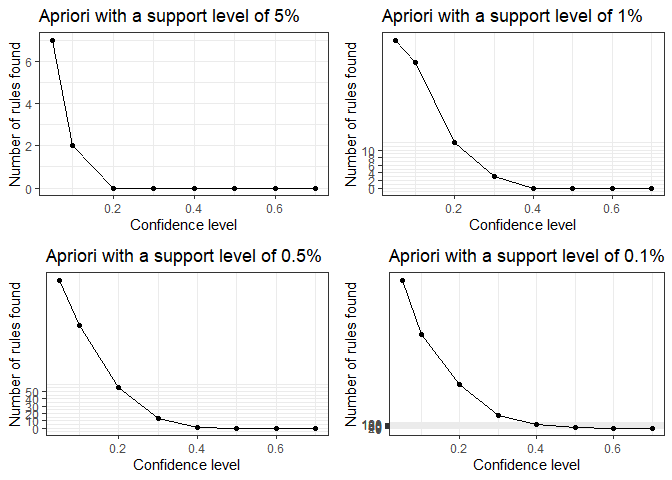
\includegraphics{Market_basket_analysis_files/figure-latex/unnamed-chunk-10-1.pdf}

\textbf{\emph{Let's plot them all together so we can compare them.}}

\begin{Shaded}
\begin{Highlighting}[]
\NormalTok{num\_rules }\OtherTok{\textless{}{-}} \FunctionTok{data.frame}\NormalTok{(rules\_sup5, rules\_sup1, rules\_sup0}\FloatTok{.5}\NormalTok{, rules\_sup0}\FloatTok{.1}\NormalTok{, confidenceLevels)}

\CommentTok{\# Number of rules found with a support level of 10\%, 5\%, 1\% and 0.5\%}
\FunctionTok{ggplot}\NormalTok{(}\AttributeTok{data=}\NormalTok{num\_rules, }\FunctionTok{aes}\NormalTok{(}\AttributeTok{x=}\NormalTok{confidenceLevels)) }\SpecialCharTok{+}
  
  \CommentTok{\# Plot line and points (support level of 10\%)}
  \FunctionTok{geom\_line}\NormalTok{(}\FunctionTok{aes}\NormalTok{(}\AttributeTok{y=}\NormalTok{rules\_sup5, }\AttributeTok{colour=}\StringTok{"Support level of 5\%"}\NormalTok{)) }\SpecialCharTok{+} 
  \FunctionTok{geom\_point}\NormalTok{(}\FunctionTok{aes}\NormalTok{(}\AttributeTok{y=}\NormalTok{rules\_sup5, }\AttributeTok{colour=}\StringTok{"Support level of 5\%"}\NormalTok{)) }\SpecialCharTok{+}
  
  \CommentTok{\# Plot line and points (support level of 5\%)}
  \FunctionTok{geom\_line}\NormalTok{(}\FunctionTok{aes}\NormalTok{(}\AttributeTok{y=}\NormalTok{rules\_sup1, }\AttributeTok{colour=}\StringTok{"Support level of 1\%"}\NormalTok{)) }\SpecialCharTok{+}
  \FunctionTok{geom\_point}\NormalTok{(}\FunctionTok{aes}\NormalTok{(}\AttributeTok{y=}\NormalTok{rules\_sup1, }\AttributeTok{colour=}\StringTok{"Support level of 1\%"}\NormalTok{)) }\SpecialCharTok{+}
  
  \CommentTok{\# Plot line and points (support level of 1\%)}
  \FunctionTok{geom\_line}\NormalTok{(}\FunctionTok{aes}\NormalTok{(}\AttributeTok{y=}\NormalTok{rules\_sup0}\FloatTok{.5}\NormalTok{, }\AttributeTok{colour=}\StringTok{"Support level of 0.5\%"}\NormalTok{)) }\SpecialCharTok{+} 
  \FunctionTok{geom\_point}\NormalTok{(}\FunctionTok{aes}\NormalTok{(}\AttributeTok{y=}\NormalTok{rules\_sup0}\FloatTok{.5}\NormalTok{, }\AttributeTok{colour=}\StringTok{"Support level of 0.5\%"}\NormalTok{)) }\SpecialCharTok{+}
  
  \CommentTok{\# Plot line and points (support level of 0.5\%)}
  \FunctionTok{geom\_line}\NormalTok{(}\FunctionTok{aes}\NormalTok{(}\AttributeTok{y=}\NormalTok{rules\_sup0}\FloatTok{.1}\NormalTok{, }\AttributeTok{colour=}\StringTok{"Support level of 0.1\%"}\NormalTok{)) }\SpecialCharTok{+}
  \FunctionTok{geom\_point}\NormalTok{(}\FunctionTok{aes}\NormalTok{(}\AttributeTok{y=}\NormalTok{rules\_sup0}\FloatTok{.1}\NormalTok{, }\AttributeTok{colour=}\StringTok{"Support level of 0.1\%"}\NormalTok{)) }\SpecialCharTok{+}
  
  \CommentTok{\# Labs and theme}
  \FunctionTok{labs}\NormalTok{(}\AttributeTok{x=}\StringTok{"Confidence levels"}\NormalTok{, }\AttributeTok{y=}\StringTok{"Number of rules found"}\NormalTok{, }
       \AttributeTok{title=}\StringTok{"Apriori algorithm with different support levels"}\NormalTok{) }\SpecialCharTok{+}
  \FunctionTok{theme\_bw}\NormalTok{() }\SpecialCharTok{+}
  \FunctionTok{theme}\NormalTok{(}\AttributeTok{legend.title=}\FunctionTok{element\_blank}\NormalTok{())}
\end{Highlighting}
\end{Shaded}

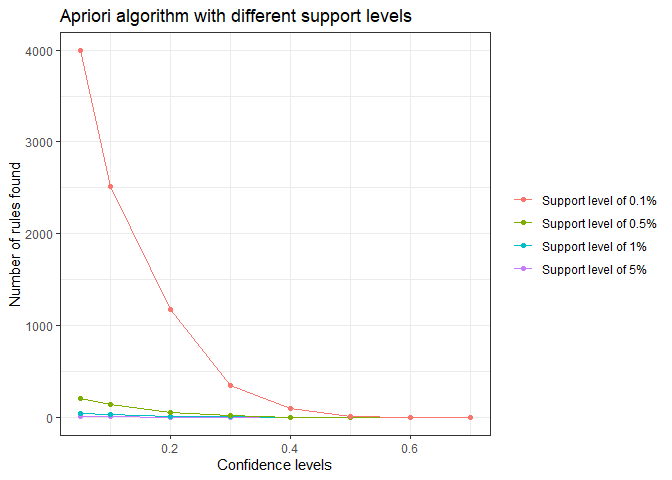
\includegraphics{Market_basket_analysis_files/figure-latex/unnamed-chunk-11-1.pdf}

\section{\texorpdfstring{\textbf{Analysis \& Association
Rules}}{Analysis \& Association Rules}}\label{analysis-association-rules}

Let's use a support level of 1\% and a confidence level of 0\% for this
analysis.
\texttt{Note:\ In\ the\ real\ world,\ this\ level\ of\ support\ and\ confidence\ may\ not\ be\ sufficient,\ and\ we\ typically\ rely\ on\ stronger\ evidence}.

\begin{Shaded}
\begin{Highlighting}[]
\NormalTok{rules }\OtherTok{\textless{}{-}} \FunctionTok{apriori}\NormalTok{(trans, }\AttributeTok{parameter=}\FunctionTok{list}\NormalTok{(}\AttributeTok{sup=}\NormalTok{supportLevels[}\DecValTok{4}\NormalTok{], }
                                                   \AttributeTok{conf=}\NormalTok{confidenceLevels[}\DecValTok{3}\NormalTok{], }\AttributeTok{target=}\StringTok{"rules"}\NormalTok{), }
                                \AttributeTok{control =} \FunctionTok{list}\NormalTok{(}\AttributeTok{verbose =} \ConstantTok{FALSE}\NormalTok{))}
\NormalTok{rules}
\end{Highlighting}
\end{Shaded}

\begin{verbatim}
## set of 11 rules
\end{verbatim}

\begin{Shaded}
\begin{Highlighting}[]
\FunctionTok{inspect}\NormalTok{(}\FunctionTok{head}\NormalTok{(rules))}
\end{Highlighting}
\end{Shaded}

\begin{verbatim}
##     lhs                                  rhs                          support confidence    coverage     lift count
## [1] {Organic Broccoli,                                                                                             
##      Organic Hass Avocado}            => {Bag of Organic Bananas} 0.001196555  0.5048232 0.002370246 4.278931   157
## [2] {Organic Hass Avocado,                                                                                         
##      Organic Unsweetened Almond Milk} => {Bag of Organic Bananas} 0.001249905  0.5141066 0.002431217 4.357618   164
## [3] {Organic Navel Orange,                                                                                         
##      Organic Raspberries}             => {Bag of Organic Bananas} 0.001150827  0.5412186 0.002126362 4.587422   151
## [4] {Organic Hass Avocado,                                                                                         
##      Organic Navel Orange}            => {Bag of Organic Bananas} 0.001493789  0.5283019 0.002827528 4.477939   196
## [5] {Organic Hass Avocado,                                                                                         
##      Organic Kiwi}                    => {Bag of Organic Bananas} 0.001448060  0.5459770 0.002652237 4.627755   190
## [6] {Organic D'Anjou Pears,                                                                                        
##      Organic Hass Avocado}            => {Bag of Organic Bananas} 0.001387089  0.5170455 0.002682722 4.382528   182
\end{verbatim}

\begin{Shaded}
\begin{Highlighting}[]
\FunctionTok{plot}\NormalTok{(rules, }\AttributeTok{measure=}\FunctionTok{c}\NormalTok{(}\StringTok{"support"}\NormalTok{, }\StringTok{"lift"}\NormalTok{), }\AttributeTok{shading=}\StringTok{"confidence"}\NormalTok{)}
\end{Highlighting}
\end{Shaded}

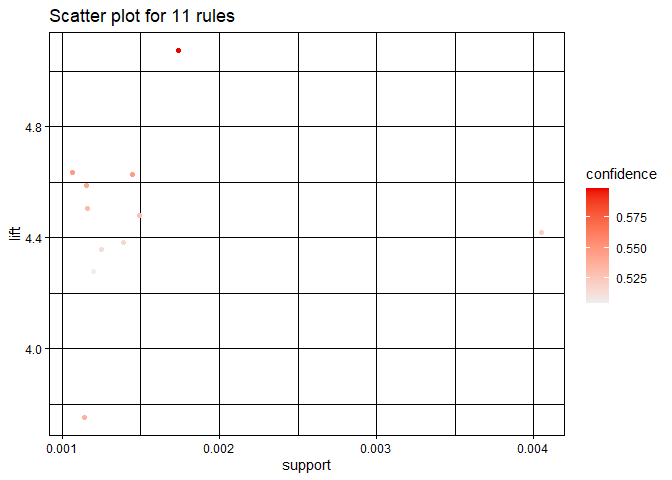
\includegraphics{Market_basket_analysis_files/figure-latex/unnamed-chunk-13-1.pdf}

\begin{Shaded}
\begin{Highlighting}[]
\FunctionTok{plot}\NormalTok{(rules, }\AttributeTok{method=}\StringTok{"graph"}\NormalTok{)}
\end{Highlighting}
\end{Shaded}

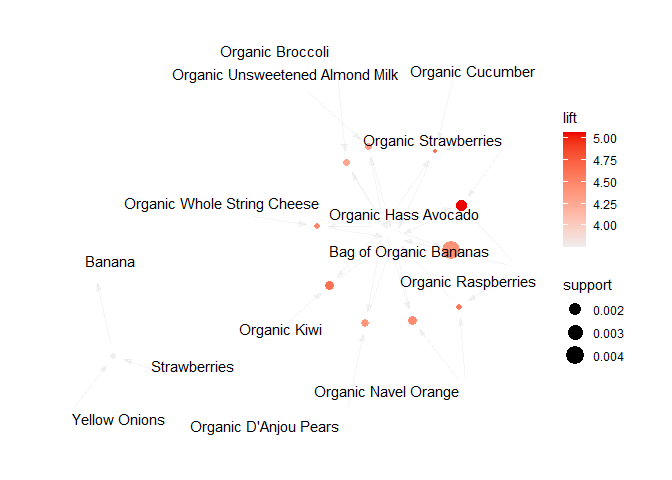
\includegraphics{Market_basket_analysis_files/figure-latex/unnamed-chunk-14-1.pdf}

\textbf{\emph{Now, I want to explore 4-product associations to determine
if purchasing products A, B, and C increases the likelihood of
purchasing product D.}}

\begin{Shaded}
\begin{Highlighting}[]
\NormalTok{rules }\OtherTok{\textless{}{-}} \FunctionTok{apriori}\NormalTok{(trans, }\AttributeTok{parameter=}\FunctionTok{list}\NormalTok{(}\AttributeTok{sup=}\NormalTok{supportLevels[}\DecValTok{4}\NormalTok{], }
                                                   \AttributeTok{conf=}\NormalTok{confidenceLevels[}\DecValTok{4}\NormalTok{],}\AttributeTok{minlen =}\DecValTok{4}\NormalTok{ , }\AttributeTok{maxlen=}\DecValTok{4}\NormalTok{, }\AttributeTok{target=}\StringTok{"rules"}\NormalTok{), }
                                \AttributeTok{control =} \FunctionTok{list}\NormalTok{(}\AttributeTok{verbose =} \ConstantTok{FALSE}\NormalTok{))}
\NormalTok{rules}
\end{Highlighting}
\end{Shaded}

\begin{verbatim}
## set of 6 rules
\end{verbatim}

\begin{Shaded}
\begin{Highlighting}[]
\FunctionTok{inspect}\NormalTok{(}\FunctionTok{head}\NormalTok{(rules))}
\end{Highlighting}
\end{Shaded}

\begin{verbatim}
##     lhs                          rhs                          support confidence    coverage     lift count
## [1] {Organic Cucumber,                                                                                     
##      Organic Hass Avocado,                                                                                 
##      Organic Strawberries}    => {Bag of Organic Bananas} 0.001066992  0.5468750 0.001951071 4.635366   140
## [2] {Organic Hass Avocado,                                                                                 
##      Organic Raspberries,                                                                                  
##      Organic Strawberries}    => {Bag of Organic Bananas} 0.001737672  0.5984252 0.002903742 5.072311   228
## [3] {Bag of Organic Bananas,                                                                               
##      Organic Hass Avocado,                                                                                 
##      Organic Raspberries}     => {Organic Strawberries}   0.001737672  0.4293785 0.004046948 5.171540   228
## [4] {Banana,                                                                                               
##      Limes,                                                                                                
##      Organic Avocado}         => {Large Lemon}            0.001112720  0.4147727 0.002682722 6.689899   146
## [5] {Large Lemon,                                                                                          
##      Organic Avocado,                                                                                      
##      Organic Baby Spinach}    => {Banana}                 0.001021264  0.4011976 0.002545538 2.811126   134
## [6] {Organic Baby Spinach,                                                                                 
##      Organic Hass Avocado,                                                                                 
##      Organic Strawberries}    => {Bag of Organic Bananas} 0.001242283  0.4939394 0.002515052 4.186679   163
\end{verbatim}

\section{\texorpdfstring{\textbf{Conclusion}}{Conclusion}}\label{conclusion}

\begin{itemize}
\item
  Using association rules we have identfied items that customers
  purchase together frequently and which products are most often
  purchased together
\item
  In addition, we have an apriori model that we can use to recommend
  instcart customer products based their existing cart !
\end{itemize}

\end{document}
